\documentclass[a4paper,12pt]{article}

\usepackage[utf8]{inputenc}
\usepackage[T2A]{fontenc}
\usepackage[english,russian]{babel}
\usepackage{amsmath,amssymb}
\usepackage{geometry}
\usepackage{graphicx}
\usepackage{booktabs}
\usepackage{longtable}
\usepackage{hyperref}

\geometry{margin=2cm}

\title{Синтез дискретных A-оптимальных планов эксперимента
для нечетких линейных двухфакторных регрессионных моделей}
\author{Вариант №28}
\date{}

\begin{document}

\begin{titlepage}
  \begin{center}
    Министерство науки и высшего образования Российской Федерации\\
    Федеральное государственное бюджетное образовательное учреждение\\
    высшего образования\\[0.5cm]
    \textbf{«Новосибирский государственный технический университет»}\\[2cm]

    Кафедра \underline{\hspace{6cm}}\\[3cm]

    \textbf{Лабораторная работа №\,\underline{\hspace{1cm}}}\\[0.5cm]
    по дисциплине «\underline{\hspace{5cm}}»\\[0.5cm]
    Тема: «Синтез дискретных A-оптимальных планов эксперимента\\
    для нечетких линейных двухфакторных регрессионных моделей»\\[3cm]

    \begin{flushright}
      Выполнил: студент гр. \underline{\hspace{2cm}}\\
      \underline{\hspace{5cm}}\\[0.5cm]
      Проверил: \underline{\hspace{5cm}}\\
    \end{flushright}

    \vfill
    Новосибирск, 2026~г.
  \end{center}
\end{titlepage}

\section{Задание}

Вариант №28. Тема: «Синтез дискретных A-оптимальных планов эксперимента
последовательным алгоритмом для нечетких линейных двухфакторных моделей».

Необходимо:
\begin{enumerate}
  \item Ознакомиться с математическим аппаратом построения регрессионных моделей
        в рамках концепции нечетких систем и с вопросами оптимального
        планирования эксперимента.
  \item Разработать программное приложение синтеза дискретных A-оптимальных
        планов эксперимента для двухфакторных нечетких регрессионных моделей.
        В качестве алгоритма использовать последовательный алгоритм достраивания.
  \item Провести численные эксперименты при
        $\delta \in \{0{,}5; 0{,}4; 0{,}3; 0{,}2\}$ на регулярной сетке $21\times 21$
        при максимальном числе точек плана $N_{\max}=60$; представить
        таблицы координат точек и графики планов.
\end{enumerate}

\section{Теоретическая часть}

В задачах идентификации и оптимального планирования эксперимента
широко применяются регрессионные модели, описывающие зависимость
выходной величины $y$ от нескольких факторов $x_1,\dots,x_m$.
Классические линейные модели предполагают чёткое задание
области факторов и единой глобальной зависимости.
Однако во многих прикладных задачах (технические системы,
социально-экономические объекты и т.\,п.)
естественно использовать \emph{нечеткие регрессионные модели},
основанные на системе нечетких правил вида
«если $x_1$~\dots, $x_2$~\dots, то $y$~\dots».

В данной работе рассматривается синтез дискретных A-оптимальных
планов эксперимента для нечеткой линейной двухфакторной модели.
В качестве метода используется последовательный алгоритм
достраивания плана на регулярной сетке $21\times 21$
на квадрате $[-1;1]\times[-1;1]$.
Фаззификация факторов выполняется с помощью двух трапециевидных
функций принадлежности для каждого фактора.
Исследуется влияние параметра фаззификации $\delta$
на характеристики A-оптимальных планов.

\subsection{Линейная нечеткая двухфакторная регрессионная модель}

\subsection{Классическая линейная модель}

Классическая двухфакторная линейная регрессионная модель имеет вид
\begin{equation}
y = \beta_0 + \beta_1 x_1 + \beta_2 x_2 + \varepsilon,
\end{equation}
где $x_1, x_2$~--- факторы, $\beta_0,\beta_1,\beta_2$~---
неизвестные параметры, $\varepsilon$~--- случайная ошибка.
В матричной форме для вектора наблюдений $y$ записывается
\begin{equation}
y = X \beta + \varepsilon,
\end{equation}
где $X$~--- матрица плана, строки которой содержат значения регрессоров
в точках эксперимента.

\subsection{Нечеткая регрессионная модель на основе правил}

В концепции нечетких систем модель представляется в виде набора правил:
\begin{align}
R_1:&\ \text{Если } x_1 \text{~--- малый и } x_2 \text{~--- малый, то }
      y = \beta_0^{(11)} + \beta_1^{(11)} x_1 + \beta_2^{(11)} x_2, \\
R_2:&\ \text{Если } x_1 \text{~--- малый и } x_2 \text{~--- большой, то }
      y = \beta_0^{(12)} + \beta_1^{(12)} x_1 + \beta_2^{(12)} x_2, \\
R_3:&\ \text{Если } x_1 \text{~--- большой и } x_2 \text{~--- малый, то }
      y = \beta_0^{(21)} + \beta_1^{(21)} x_1 + \beta_2^{(21)} x_2, \\
R_4:&\ \text{Если } x_1 \text{~--- большой и } x_2 \text{~--- большой, то }
      y = \beta_0^{(22)} + \beta_1^{(22)} x_1 + \beta_2^{(22)} x_2.
\end{align}

Каждое правило определяет \emph{локальную} линейную модель в определённой
области пространства факторов. Степень влияния правила при конкретных
значениях $x_1,x_2$ определяется величинами степеней принадлежности
этих значений соответствующим нечетким термам.

Пусть для фактора $x_1$ заданы две нечеткие партиции с функциями
принадлежности $\mu_1(x_1)$ и $\mu_2(x_1)$,
аналогично для $x_2$~--- $\mu_1(x_2)$ и $\mu_2(x_2)$.
Тогда веса правил вычисляются как
\begin{align}
w_{11} &= \mu_1(x_1) \mu_1(x_2), \\
w_{12} &= \mu_1(x_1) \mu_2(x_2), \\
w_{21} &= \mu_2(x_1) \mu_1(x_2), \\
w_{22} &= \mu_2(x_1) \mu_2(x_2).
\end{align}
Итоговый выход модели определяется агрегированием по всем правилам:
\begin{equation}
y(x_1,x_2) =
\sum_{i=1}^{2} \sum_{j=1}^{2}
w_{ij}(x_1,x_2)
\left(
\beta_0^{(ij)} + \beta_1^{(ij)} x_1 + \beta_2^{(ij)} x_2
\right).
\end{equation}

Таким образом, модель остаётся линейной по параметрам
$\beta^{(ij)}_k$, но учитывает нелинейный характер влияния
факторов за счёт нечеткого разбиения области определения.

\subsection{Фаззификация и трапециевидные нечеткие партиции}

\subsection{Понятие фаззификации}

\emph{Фаззификация} (fuzzification)~--- это переход от чётких значений
входных величин к их нечеткому представлению.
Каждому значению $x$ сопоставляется вектор степеней принадлежности
к нескольким нечетким термам:
\begin{equation}
x \mapsto \bigl( \mu_1(x), \mu_2(x), \dots, \mu_K(x) \bigr),\quad
\mu_k(x) \in [0,1].
\end{equation}
При этом одно и то же значение может частично принадлежать сразу
нескольким термам (например, «немного малый» и «немного большой»).

\subsection{Трапециевидные функции принадлежности}

В задании область определения каждого фактора $x_i$
равна отрезку $[-1;1]$, который разбивается на две трапециевидные
нечеткие партиции с функциями принадлежности
$\mu_1(x)$ и $\mu_2(x)$ следующего вида:
\begin{equation}
\mu_1(x) =
\begin{cases}
1, & x \le -\delta, \\
\dfrac{\delta - x}{2\delta}, & -\delta \le x \le \delta, \\
0, & x > \delta,
\end{cases}
\qquad
\mu_2(x) = 1 - \mu_1(x),
\end{equation}
где $\delta>0$~--- параметр ширины переходной области.
Для малых $|x|$ значения $\mu_1$ и $\mu_2$
плавно изменяются от 1 до 0, обеспечивая «мягкое»
разделение области факторов на две партиции.

В работе рассматриваются значения
\[
\delta \in \{0{,}5;\ 0{,}4;\ 0{,}3;\ 0{,}2\},
\]
что позволяет исследовать влияние степени «размытия» разбиения
на свойства A-оптимального плана.

\subsection{Информационная матрица и критерий A-оптимальности}

\subsection{Вектор регрессоров}

Для каждой точки плана $(x_1,x_2)$ формируется 12-мерный вектор
регрессоров, соответствующий четырём нечетким правилам и трём
регрессорам в каждом правиле:
\begin{equation}
f(x_1,x_2) =
\bigl[
w_{11}, w_{11}x_1, w_{11}x_2,\;
w_{12}, w_{12}x_1, w_{12}x_2,\;
w_{21}, w_{21}x_1, w_{21}x_2,\;
w_{22}, w_{22}x_1, w_{22}x_2
\bigr]^T.
\end{equation}
Всего в модели $4 \times 3 = 12$ параметров.

\subsection{Информационная матрица}

Пусть план эксперимента состоит из набора точек
\[
\xi = \{(x_1^{(k)}, x_2^{(k)})\}_{k=1}^N,
\quad N \le 60.
\]
Информационная матрица модели определяется как
\begin{equation}
M(\xi) = \sum_{k=1}^{N}
f(x_1^{(k)}, x_2^{(k)})\,
f(x_1^{(k)}, x_2^{(k)})^T.
\end{equation}
Размерность $M$ равна $12\times 12$.
При предположении о нормальности ошибок
оценка дисперсионной матрицы вектора оценок параметров
пропорциональна $M^{-1}$.

\subsection{Критерий A-оптимальности}

Критерий A-оптимальности направлен на минимизацию суммарной дисперсии
оценок параметров и определяется как
\begin{equation}
\Phi_A(\xi) = \mathrm{tr}\,\bigl( M(\xi)^{-1} \bigr).
\end{equation}
В реализации для устойчивости при малом числе точек используется
регуляризованный вариант
\begin{equation}
\Phi_A^{\text{reg}}(\xi) =
\mathrm{tr}\,\bigl( (M(\xi) + \lambda I)^{-1} \bigr),
\end{equation}
где $\lambda = 10^{-8}$, $I$~--- единичная матрица.
На финальном шаге, при $N=60$, матрица $M$ невырождена
(ранг 12), поэтому регуляризация практически не влияет на результат.

\subsection{Последовательный алгоритм достраивания плана}

Для синтеза дискретного A-оптимального плана используется
последовательный алгоритм достраивания:

\begin{enumerate}
\item Задаётся дискретная область планирования~--- регулярная сетка
      $21\times 21$ на квадрате $[-1;1]\times[-1;1]$.
      Максимальное число точек плана $N_{\max}=60$.

\item Начинаем с пустого плана:
      $M_0 = 0$, $\,\xi_0 = \varnothing$.

\item На $t$-м шаге ($t=0,1,\dots,N_{\max}-1$) для
      каждой ещё не выбранной точки $(x_1,x_2)$ сетки
      вычисляется \emph{кандидатная} информационная матрица
      \begin{equation}
      M_{\text{cand}} = M_t + f(x_1,x_2) f(x_1,x_2)^T
      \end{equation}
      и значение A-критерия
      $\Phi_A^{\text{reg}}(M_{\text{cand}})$.

\item Выбирается точка, дающая минимальное значение критерия:
      \begin{equation}
      (x_1^{*},x_2^{*}) =
      \arg\min_{(x_1,x_2)\in G \setminus \xi_t}
      \Phi_A^{\text{reg}}\bigl(M_t + f f^T\bigr),
      \end{equation}
      где $G$~--- множество всех узлов сетки.

\item Обновляются матрица и план:
      \begin{equation}
      M_{t+1} = M_t + f(x_1^{*},x_2^{*}) f(x_1^{*},x_2^{*})^T,\quad
      \xi_{t+1} = \xi_t \cup \{(x_1^{*},x_2^{*})\}.
      \end{equation}

\item Процесс повторяется до достижения $|\xi_t| = N_{\max}=60$.
\end{enumerate}

Алгоритм реализует жадное достраивание плана и является
стандартным подходом к построению дискретных A-оптимальных планов
(см., например, работы А.\,А.~Попова по оптимальному планированию
эксперимента для нечетких регрессионных моделей).

% Раздел с описанием программной реализации приведён ниже,
% после результатов экспериментов.

\section{Результаты численных экспериментов}

\subsection{Тестовые примеры}

В соответствии с заданием проведены эксперименты для
\[
\delta \in \{0{,}5;\ 0{,}4;\ 0{,}3;\ 0{,}2\},
\]
область факторов $x_1,x_2 \in [-1;1]$,
область планирования~--- регулярная сетка $21\times 21$,
максимальное число точек в плане $N_{\max} = 60$.

Для каждого значения $\delta$ был синтезирован дискретный
A-оптимальный план из 60 точек и вычислены характеристики
информационной матрицы $M$:
след A-обратной матрицы, детерминант, ранг и число обусловленности.

\subsection{Численные характеристики матрицы $M$}

Сводная таблица результатов:

\begin{table}[h!]
\centering
\caption{Характеристики информационной матрицы $M$ для различных $\delta$}
\begin{tabular}{cccccc}
\toprule
$\delta$ &
$\mathrm{tr}(M^{-1})$ &
$\det(M)$ &
\rule{0pt}{2.4ex}ранг &
$\mathrm{cond}(M)$ \\
\midrule
0.5 & $1.347093 \cdot 10^{1}$ & $1.785608 \cdot 10^{4}$ &
12 & $8.880044 \cdot 10^{1}$ \\
0.4 & $9.990348 \cdot 10^{0}$ & $1.144807 \cdot 10^{5}$ &
12 & $6.024355 \cdot 10^{1}$ \\
0.3 & $7.572914 \cdot 10^{0}$ & $8.638962 \cdot 10^{5}$ &
12 & $3.425808 \cdot 10^{1}$ \\
0.2 & $5.736220 \cdot 10^{0}$ & $6.686027 \cdot 10^{6}$ &
12 & $2.397692 \cdot 10^{1}$ \\
\bottomrule
\end{tabular}
\end{table}

Из таблицы видно, что при уменьшении параметра фаззификации $\delta$
значение критерия A-оптимальности $\mathrm{tr}(M^{-1})$ монотонно
уменьшается, а детерминант матрицы $M$ существенно возрастает.
Число обусловленности $ \mathrm{cond}(M)$ также уменьшается,
что свидетельствует о лучшей численной устойчивости оценки параметров.
Во всех случаях ранг матрицы равен 12, то есть вся совокупность
параметров нечеткой регрессионной модели идентифицируема.

\subsection{Графическое расположение точек планов}

На рисунках~\ref{fig:delta05}--\ref{fig:delta02}
представлены графики расположения точек A-оптимальных планов
для различных значений параметра $\delta$.
Каждый план содержит 60 точек на квадрате $[-1;1]\times[-1;1]$.

\begin{figure}[h!]
\centering
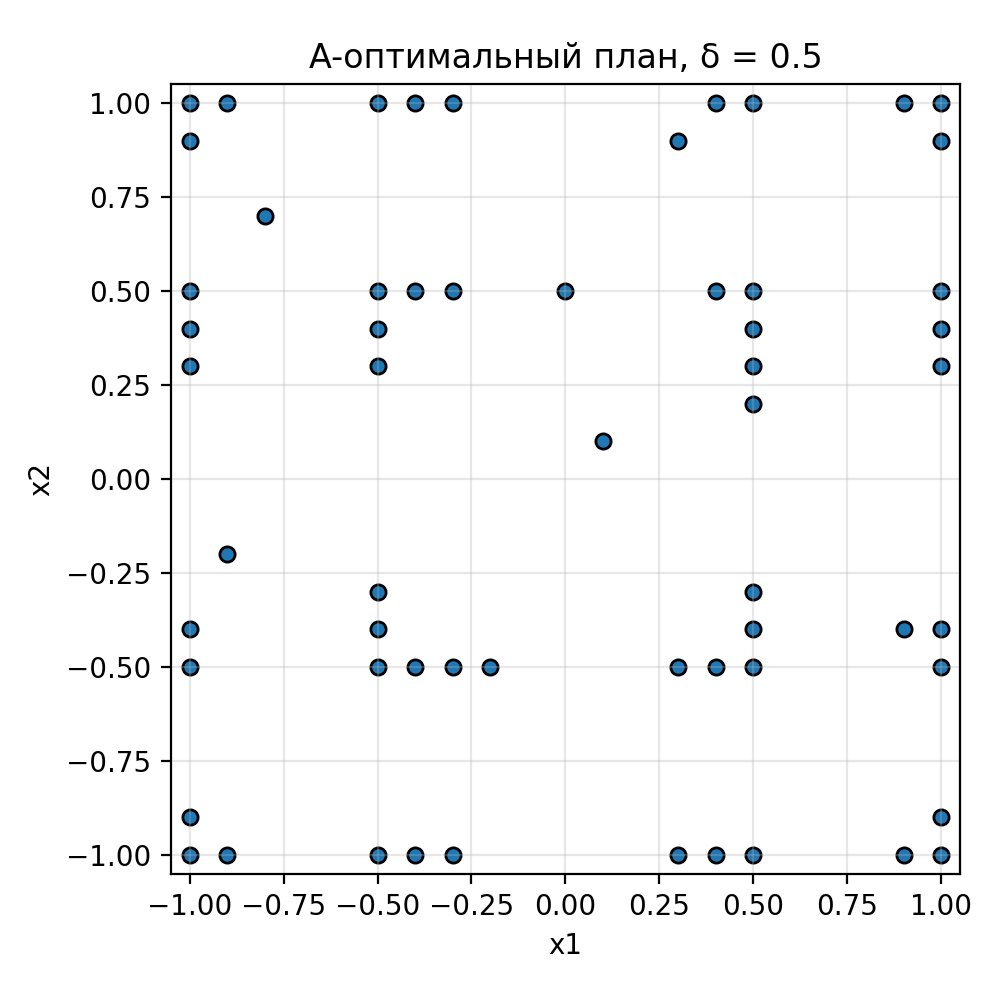
\includegraphics[width=0.45\textwidth]{plan_delta_0.50.png}
\caption{A-оптимальный план при $\delta = 0{,}5$}
\label{fig:delta05}
\end{figure}

\begin{figure}[h!]
\centering
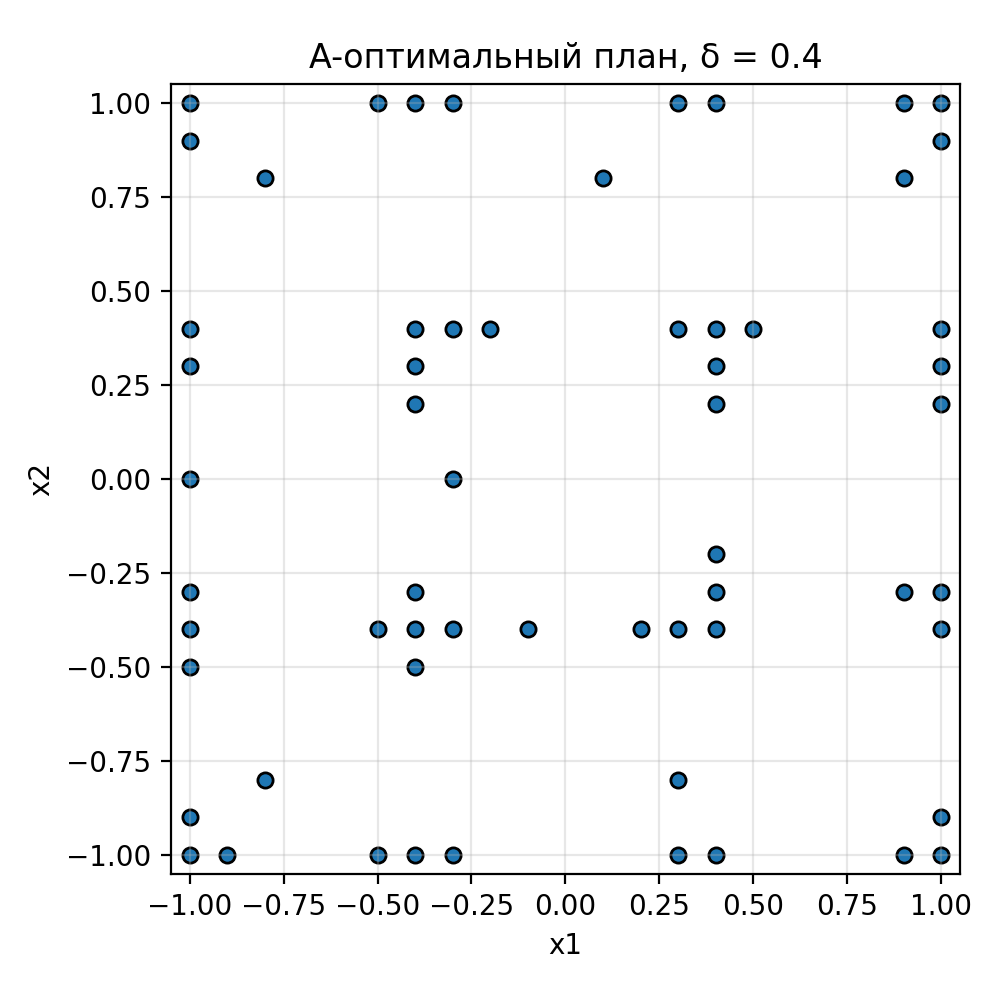
\includegraphics[width=0.45\textwidth]{plan_delta_0.40.png}
\caption{A-оптимальный план при $\delta = 0{,}4$}
\label{fig:delta04}
\end{figure}

\begin{figure}[h!]
\centering
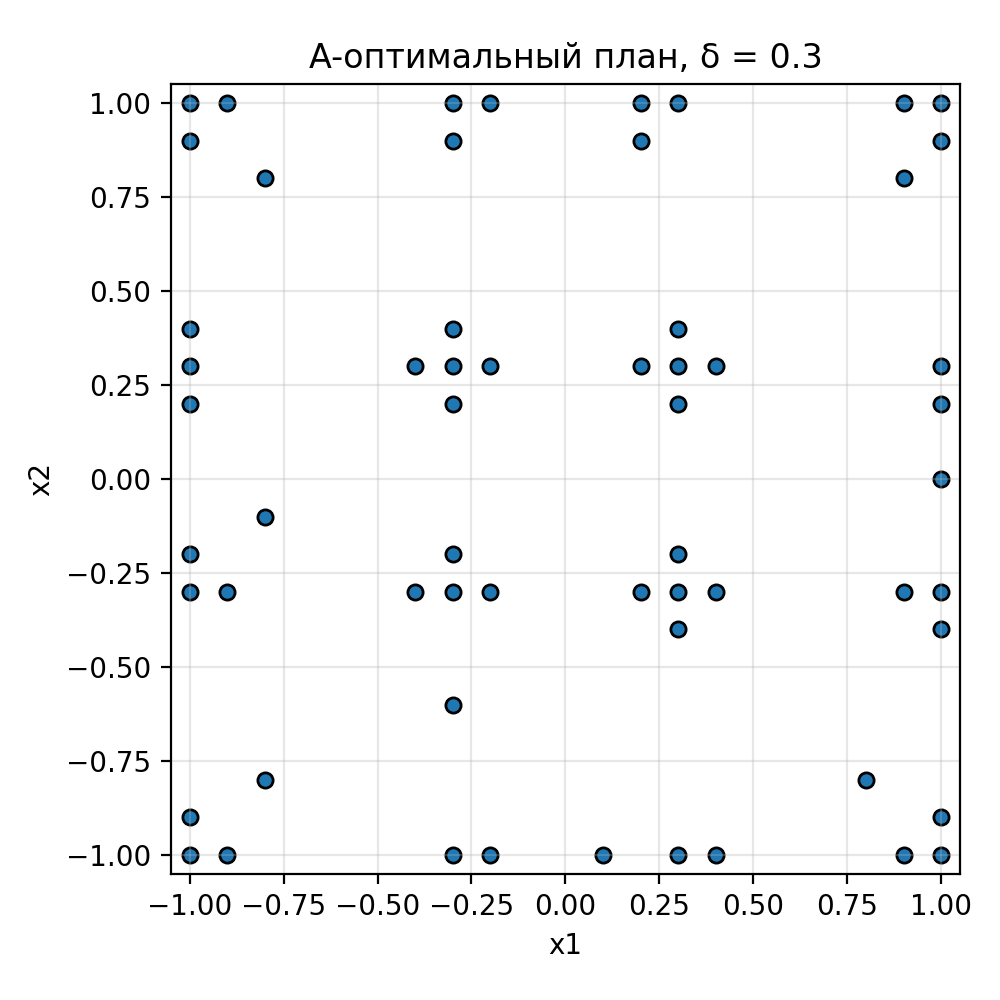
\includegraphics[width=0.45\textwidth]{plan_delta_0.30.png}
\caption{A-оптимальный план при $\delta = 0{,}3$}
\label{fig:delta03}
\end{figure}

\begin{figure}[h!]
\centering
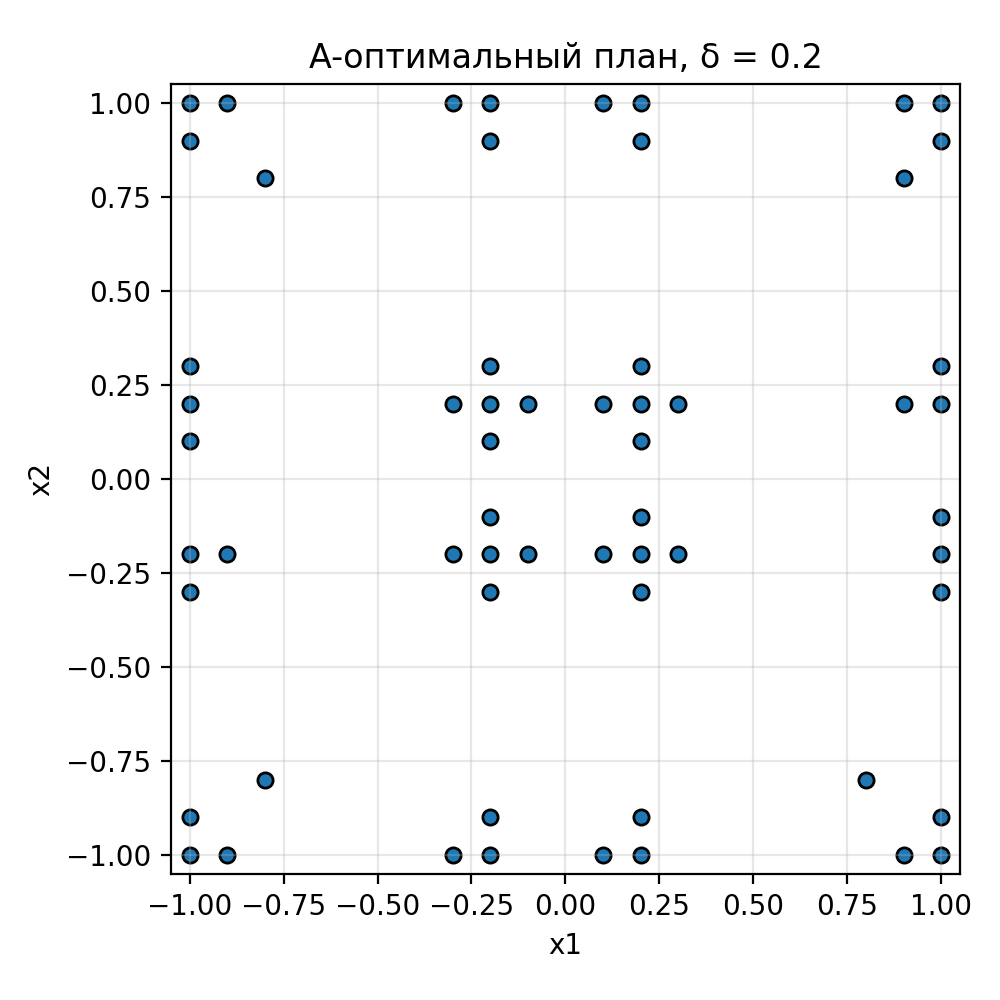
\includegraphics[width=0.45\textwidth]{plan_delta_0.20.png}
\caption{A-оптимальный план при $\delta = 0{,}2$}
\label{fig:delta02}
\end{figure}

Визуальный анализ показывает, что точки планов концентрируются
вблизи границ и в окрестности нуля, обеспечивая хороший баланс
между глобальным покрытием области факторов и точностью оценивания
параметров в наиболее информативных зонах.

\subsection{Координаты точек планов}

Координаты точек синтезированных планов для каждого значения $\delta$
были получены непосредственно из работы программы.
Ниже при необходимости могут быть приведены полные таблицы координат
точек планов для всех четырёх значений параметра $\delta$
(по 60 строк на каждый план), используя среду \texttt{longtable}.

% Здесь при необходимости можно вставить longtable с полным списком
% точек для каждого значения \delta, используя вывод программы.

\section{Программная реализация}

Приложение реализовано на языке \texttt{Python} с использованием
библиотек \texttt{NumPy} и \texttt{Matplotlib}.
Структура исходного кода:

\begin{itemize}
\item Файл \texttt{src/fuzzy.py}:
      функции фаззификации и формирования регрессора.
\item Файл \texttt{src/model.py}:
      генерация сетки, вычисление информационной матрицы,
      реализация алгоритма синтеза, расчёт характеристик матрицы,
      построение графиков и вывод таблиц.
\end{itemize}

Основные функции:

\begin{itemize}
\item \texttt{mu1(x, delta)}, \texttt{mu2(x, delta)}~---
      трапециевидные функции принадлежности для фаззификации факторов.
\item \texttt{fuzzy\_weights(x1, x2, delta)}~---
      вычисление весов правил $w_{11}, w_{12}, w_{21}, w_{22}$.
\item \texttt{regressor\_vector(x1, x2, delta)}~---
      формирование 12-мерного вектора регрессоров $f(x)$.
\item \texttt{compute\_info\_matrix(points, delta)}~---
      вычисление информационной матрицы $M$ для заданного набора точек.
\item \texttt{synthesize\_a\_optimal\_plan(delta, grid, max\_points)}~---
      реализация последовательного алгоритма достраивания.
\item \texttt{analyze\_matrix(M)}~---
      расчёт $\mathrm{tr}(M^{-1})$, $\det(M)$, ранга и числа обусловленности.
\item \texttt{plot\_plan(points, delta)}~---
      построение и сохранение графика расположения точек плана.
\item \texttt{run\_synthesis\_for\_deltas()}~---
      запуск экспериментов для $\delta \in \{0{,}5;0{,}4;0{,}3;0{,}2\}$.
\end{itemize}

Запуск приложения осуществляется командой
\begin{verbatim}
python -m src.model
\end{verbatim}
из корневой директории проекта. По завершении работы для каждого
значения $\delta$ выводятся таблицы координат точек плана
и численные характеристики матрицы $M$, а также сохраняются
рисунки с расположением точек в файлы
\texttt{plan\_delta\_0.50.png},
\texttt{plan\_delta\_0.40.png},
\texttt{plan\_delta\_0.30.png},
\texttt{plan\_delta\_0.20.png}.

\section*{Заключение}

В работе разработано и реализовано программное приложение
для синтеза дискретных A-оптимальных планов эксперимента
для нечеткой линейной двухфакторной регрессионной модели
на основе последовательного алгоритма достраивания плана
на регулярной сетке.

Проведённые численные эксперименты для значений
$\delta \in \{0{,}5;\ 0{,}4;\ 0{,}3;\ 0{,}2\}$
показывают, что при уменьшении параметра фаззификации
улучшаются характеристики A-оптимального плана:
уменьшается значение $\mathrm{tr}(M^{-1})$,
возрастает детерминант $M$ и снижается число обусловленности.
Полученные результаты согласуются с теоретическими представлениями
об оптимальном планировании эксперимента для нечетких моделей.

\section*{Литература}

\begin{enumerate}
\item Попов А.\,А. Регрессионное моделирование на основе нечетких правил~//
      Сборник научных трудов НГТУ. 2000. №\,2(19). С.~49--57.
\item Пегат А. Нечеткое моделирование и управление. 2-е изд. М.:
      БИНОМ. Лаборатория знаний, 2013. 798~с.
\item Попов А.\,А. Планирование и анализ эксперимента. Конспект лекций.
      Электронный вариант.
\item Попов А.\,А. Оптимальное планирование эксперимента в задачах структурной
      и параметрической идентификации моделей многофакторных систем:
      монография. Новосибирск: Изд-во НГТУ, 2013. 296~с.
\item Попов А.\,А. Оптимальное планирование эксперимента при активной
      идентификации нечетких линейных регрессионных моделей~//
      Modeling, Optimization and Information Technology. 2019. Т.~7, №\,1.
\item Халов Е.\,Л. Систематический обзор чётких одномерных функций
      принадлежности интеллектуальных систем.
\end{enumerate}

\end{document}